%----------------------------------------------------------------------------------------
%	PACKAGES AND DOCUMENT CONFIGURATIONS
%----------------------------------------------------------------------------------------

\documentclass[letter, 10pt]{article}

\usepackage{fancyhdr, graphicx, float} % Required for the inclusion of images
\usepackage{amsmath} % Required for some math elements
\newcommand{\BigO}[1]{\ensuremath{\operatorname{O}\bigl(#1\bigr)}}
\usepackage{mathtools}
\usepackage{tikz} % Required for generate trees
\usetikzlibrary{trees,positioning}
\usepackage{listings}

\usepackage[spanish]{babel} % Para separar correctamente las palabras
\usepackage[utf8]{inputenc} % Este paquete permite poner acentos y eñes usando c

\usepackage[titletoc,toc,title]{appendix}

\setlength\parindent{0pt} % Removes all indentation from paragraphs

\renewcommand{\labelenumi}{\alph{enumi}.} % Make numbering in the enumerate environment by letter rather than number (e.g. section 6)

%\usepackage{times} % Uncomment to use the Times New Roman font

%----------------------------------------------------------------------------------------
%	DOCUMENT INFORMATION
%----------------------------------------------------------------------------------------

\textheight=21cm
\textwidth=16.5cm
\topmargin=-0.5cm
\oddsidemargin=0cm
\parindent=0mm

\renewcommand{\headrulewidth}{0pt}
\fancyhead[L]{
\includegraphics[width=5em]{images/logo_c_ucn_small}\hspace{0.3cm}\parbox[b][4em][t]{0.8\textwidth}{Universidad Católica del Norte \\ Departamento de Ingeniería de Sistemas y Computación \\ Magíster en Ingeniería Informática}}
\fancyhead[R]{}

\title{TAREA 2: \\ Ocho Reinas \\ Resolución de Problemas Basados en Búsqueda} % Title
\date{15 de Mayo, 2014}

\begin{document}

\maketitle % Insert the title, author and date
\thispagestyle{fancy}

\begin{center}
\begin{tabular}{l r}
Fecha de Entrega: &  15 de Mayo, 2014 \\ % Date the experiment was performed
Autor: & Exequiel Fuentes Lettura \\
Asignatura: & Sistemas Inteligentes\\ % Asignatura
Profesor: & Juan Bekios-Calfa % Instructor/supervisor
\end{tabular}
\end{center}

% If you wish to include an abstract, uncomment the lines below
% \begin{abstract}
% Abstract text
% \end{abstract}

%----------------------------------------------------------------------------------------
%	SECTION 1
%----------------------------------------------------------------------------------------

\section{Introducción}

El problema de las 8 Reinas fue propuesto por el entusiasta ajedrecista Max Bezzel en 1848. Este consiste en situar 8 Reinas en un tablero de ajedrez de 8x8 sin que ninguna Reina se ataque \cite[pág 71]{Russell10}. Una Reina ataca a otra Reina cuando se encuentra en la misma fila, columna o en diagonal. La figura~\ref{fig:mov_queen} muestra los posibles movimientos de una Reina.

\begin{figure}[H]
    \begin{center}
        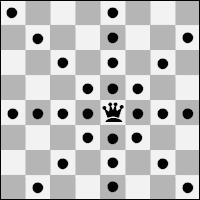
\includegraphics[width=100px,height=100px,keepaspectratio]{images/reinamueve}
        \caption{Movimientos de una Reina}
        \label{fig:mov_queen}
    \end{center}
\end{figure}

Entonces, dado un tablero de 8x8 debemos situar las 8 Reinas sin que ninguna ellas coincida en fila, columna o en diagonal, la figura~\ref{fig:8queens} muestra una de las 92 soluciones al problema de las 8 Reinas.

\begin{figure}[H]
    \begin{center}
        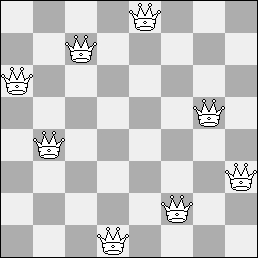
\includegraphics[width=100px,height=100px,keepaspectratio]{images/8queens}
        \caption{Una de las 92 soluciones al problema}
        \label{fig:8queens}
    \end{center}
\end{figure}

El estado inicial es un tablero vacío, la inserción de la primera Reina no requiere comparaciones, a diferencia de las siguientes inserciones que requieren verificar la regla del juego. La figura~\ref{fig:queen_tree} muestra el árbol de tableros que se va generando en la medida que se va insertando una Reina en el tablero. Nótese que cada nivel representa todas las posibles posiciones de las Reinas. Si una configuración de un tablero no es válido este será eliminado. Un tablero hoja con las 8 Reinas con posiciones validas será una solución.

\begin{figure}[H]
    \centering
        \begin{tikzpicture}
            \node (a) {$T_{0}$}
                child {
                    node (b) {$T_{0.0}$}
                    child {
                        node (ba) {$T_{1.0}$} 
                    }
                    child {
                        node (ba) {...} 
                    }
                    child {
                        node (ba) {$T_{1.7}$} 
                    }
                }
                child {
                    node (c) {$T_{0.1}$}
                }
                child {
                    node (d) {...}
                }
                child {
                    node (e) {$T_{0.7}$}
                };
            \begin{scope}[every node/.style={font=\footnotesize,color=black}]
                \node[right=of a] (na) {\{Tablero inicial vacío\}};
                \node[right=of e] (ne) {\{Diferentes posiciones de la primera Reina\}};
                \node[right=of ba] (nba) {\{Diferentes posiciones de la segunda Reina\}};
                \foreach \i in {a,e,ba}
                    \draw[dotted] (\i) -- (n\i);
            \end{scope}
        \end{tikzpicture}
    \caption{Árbol de tableros. Índices indican posición de la Reina en el tablero}
    \label{fig:queen_tree}
\end{figure}

Este problema puede ser resuelto a través de varias metodologías. Este estudio particularmente utiliza tres algoritmos de búsqueda para localizar las soluciones: 1. Breadth-First Search, 2. Depth-First Search y 3. Iterative Deepening Depth-First Search. Cada uno de estos algoritmos de búsqueda utiliza una estructura de datos especifica para buscar la propiedad deseada en el tablero.

% Definir los objetivos en esta seccion
\subsection{Objetivos}

\begin{description}
    \item[Primer Objetivo] \hfill \\
    El objetivo principal de este estudio es modelar y formular una solución al problema de las 8 Reinas usando los algoritmos de búsqueda seleccionados.
    \item[Segundo Objetivo] \hfill \\
    El segundo objetivo es determinar la eficiencia de los algoritmos implementados.
\end{description}


%----------------------------------------------------------------------------------------
%	SECTION 2
%----------------------------------------------------------------------------------------

\section{Métodos implementados}

Primero, el algoritmo de búsqueda debe ser diseñado para buscar un tablero que satisfaga las condiciones del juego, esto es que ninguna de las 8 Reinas pueda atacarse. Por ejemplo, $R_{1}$ inicialmente no ataca a ninguna pieza porque es la única en el tablero, entonces se inserta en cualquier columna de la primera fila. Cuando se quiere insertar $R_{2}$ primero se debe verificar en que columna de la segunda fila puede insertarse para cumplir con la regla, eso debería ser algo mas o menos sencillo. Ahora, insertar la siguiente $R_{3}$ en la tercera fila es algo mas difícil, ya que no debe atacar a $R_{1}$ y $R_{2}$. Es posible que al insertar $R_{3}$ y/o las siguientes piezas sea imposible con la configuración del tablero actual, entonces se debe volver al estado en que las Reinas en el tablero son válidas descartando la configuración no válida. Considerando lo anterior, los siguientes métodos de búsqueda serán utilizados.

\subsection{Algoritmos de Búsqueda}

En general, un algoritmo de búsqueda toma un estado inicial y retorna una solución del espacio de búsquedas. El espacio de búsquedas es un conjunto de todas las posibles soluciones. Para encontrar el estado final debemos recorrer desde un estado inicial hasta el estado final de meta, a este camino se le denomina espacio de estados. Es útil pensar en la búsqueda como la construcción de un árbol como muestra la figura~\ref{fig:queen_tree}. Entonces, básicamente la solución en pseudocódigo usando algoritmos de búsqueda sería: \\

\begin{lstlisting}[frame=single]
    # Creacion del tablero inicial
    estado_inicial <- tablero.nuevo()
    # Dependiendo del tipo de algoritmo de búsqueda que se use
    # debe ser elegida la estructura de datos
    estados_abiertos <- cola.nuevo() # pila.nuevo()
    While length(estados_abiertos) != 0
        tablero_actual <- estados_abierto.pop()
        If tablero_actual <- es valido?
            Imprimir <- tablero_actual
        Else
            nuevos_tableros <- generar_nuevos_tableros()
            estados_abiertos <- agregar nuevos_tableros
\end{lstlisting}

\subsubsection{Definición formal del problema}

Primero, definamos nuestras reglas:
\begin{enumerate}
    \item 2 Reinas no pueden estar en la misma fila
    \item 2 Reinas no pueden estar en la misma columna
    \item 2 Reinas no pueden estar en la misma celda
    \item 2 Reinas no pueden estar en la misma diagonal
\end{enumerate}

Las reglas a, b y c pueden ser formalmente definidas como:
\begin{align*}
    \forall i, j; &\quad R_{i} \neq R_{j}
\end{align*}

Y la regla d puede ser formalizada:
\begin{align*}
    \forall i, j; Si R_{i} = x y R_{j} = y \\
    Entonces i - j \neq y - x
\end{align*}

Ahora, el tablero inicial debe ser vacío, por lo tanto:
\begin{align*}
    T_{0} = \emptyset
\end{align*}

Un tablero que cumpla con todas las reglas debe ser de la siguiente forma:
\begin{align*}
    T_{f} = {R_{1}, R_{2},\ldots, R_{n}} \\
    Donde 1 \leq n \leq 8 y f es nuestro tablero final
\end{align*}

Entonces, nuestro espacio de soluciones se definiría como:
\begin{align*}
    S = {T_{f1}, T_{f2},\ldots, T_{fk}}\\
    \text{Donde k son todas las soluciones válidas}
\end{align*}

\begin{description}
    \item[Estado Inicial] \hfill \\
    Como se ha mencionado, el estado inicial será un tablero vacío, esto es 0 Reinas en el tablero. Un tablero lleno será un tablero con las 8 Reinas en una posición valida.
    \item[Acciones] \hfill \\
    Tenemos las siguientes acciones definidas para este problema: \\
    1. Insertar Reinas si esta cumple con las reglas definidas anteriormente.\\
    2. Generar los siguientes sucesores.
    \item[Modelo de transición] \hfill \\
    Para el estado inicial, siguiendo la acción 1, tendremos la primera Reina insertada en cualquiera columna de la fila 1. Entonces, tendremos un tablero con una Reina. Ahora, el siguiente paso es la generación de los sucesores. Nuestro modelo deberá retornar todos los posibles tableros donde la segunda Reina haya sido insertada en la segunda fila siguiendo las reglas del juego. Y así sucesivamente hasta conseguir el objetivo.
    \item[Prueba de meta (objetivo)] \hfill \\
    El objetivo será alcanzado cuando se haya insertado las 8 Reinas en el tablero. Nótese que al llegar al tablero con las 8 Reinas ya insertadas este será válido porque el modelo de transición permite sólo insertar una Reina si esta cumple con las reglas del juego.
    \item[Costo del Camino] \hfill \\
    El costo del camino puede ser medido en término de movimientos porque no tenemos información adicional de los costos asociados a búsqueda. Entonces, podríamos asignarle el valor 1 a cada movimiento. Este valor puede contarse cada vez que se genere los nuevos sucesores. \\

\subsubsection{Explicación de los algoritmos de búsqueda}

El problema se resolvió a través de 3 algoritmos de búsqueda:

1. Breadth-First Search \\
Comienza con el tablero raíz, en este caso un tablero vacío. Luego, se exploraría sus nodos vecinos, pero como es la raíz entonces descendería a través de sus hijos. A continuación para cada uno de los vecinos se exploran sus respectivos vecinos adyacentes, y así hasta que se recorra todo el árbol. Esto es realizado a través de una cola (FIFO). Es una búsqueda exhaustiva, esto significa que termina hasta recorrer todo el árbol. \\

2. Depth-First Search \\
Al igual que Breadth-First Search, este algoritmo comienza con un tablero vacío. A diferencia de Breadth-First Search, este se va expandiendo por cada nodo hijo de forma recurrente. Cuando no encuentra más nodos que visitar, entonces regresa al padre y visita el siguiente hijo, así repitiendo el mismo proceso. Esto es realizado a través de una pila (LIFO). Y de la misma manera, es una búsqueda exhaustiva, esto significa que termina hasta recorrer todo el árbol. \\

3. Iterative Deepening Depth-First Search \\
Básicamente es la misma implementación que Depth-First Search, la única diferencia que se agrega un límite de carácter constante a las búsquedas. Se inicia con un valor 0 y se va incrementando gradualmente en la medida que necesita internarse en el árbol. Es posible que no encuentre una solución para el límite dado.

\end{description}

\subsection{Código Documentado}

A continuación se adjunta las partes esenciales del código. Se utilizo Orientación a Objetos para modelar el tablero y la Reina.\\

La clase Reina esta definida de la siguiente manera: \\

\begin{lstlisting}[language=python,frame=single]
    class Queen:
    """La clase Queen representa a una reina"""

    def __init__(self):
        """Crea una instancia de la clase Queen."""
        self.row = -1
        self.column = -1

    def is_valid(self):
        """Verifica si la reina tiene asignada una posicion"""
        if self.row != -1 and self.column != -1:
            return True
        else:
            return False

    def is_attacking(self, queen):
        """Determina si la actual reina esta atacando a la reina pasada

        :param queen: La reina a comparar con la actual reina
        """
        if self.row == queen.row or self.column == queen.column: return True
        if abs(self.row-queen.row) == abs(self.column-queen.column): return True
        return False
\end{lstlisting}

La clase Tablero esta definida como:\\

\begin{lstlisting}[language=python,frame=single]
    class Board:
    """La clase Board representa al tablero"""
    def __init__(self, board_size):
        """Crea una instancia de Board.
    
        :param board_size: Tamano del tablero
        """
        self.board_size = board_size
        self.queens = []
        self.depth_index = 0 # indica la profundidad en el arbol
    
    def set_queen(self, row, column):
        """Asigna una posicion a la reina si no ataca a otra

        :param row: Fila en el tablero
        :param column: Columns en el tablero
        """
        tmp_queen = Queen()
        tmp_queen.row = row
        tmp_queen.column = column

        for queen in self.queens:
            if queen.is_valid() and tmp_queen.is_attacking(queen):
                return False

        self.queens.append(tmp_queen)

        return True
    
    def is_valid(self):
        """Verifica si el tablero es valido"""
        if len(self.queens) == self.board_size: return True
        return False
\end{lstlisting}

Luego, se definio una clase general llamada Queens para generar los sucesores e implementar los algoritmos de búsqueda.\\

\begin{lstlisting}[language=python,frame=single]
    class Queens:
    """La clase Queens define varios metodos para resolver el problem de 
    las 8 reinas. Esta solucion comienza con un tablero vacio, en cada 
    action se agrega unareina al tablero si esta no ataca a las otras reinas.
    """

    def __init__(self, options):
        """Crea una instancia de la clase Queens

        :param options: Valores opcionales para inicializar las variables 
        de clase
        """
        self.board_size = 8
        self.options = options
    
    def __get_successors(self, current_board):
        """Retorna los siguientes sucesores

        :param current_board: Es el actual tablero
        """
        new_board_successors = []

        for col in xrange(self.board_size):
            board_successor = copy.deepcopy(current_board)
            if board_successor.set_queen(board_successor.get_depth(), col):
                board_successor.increment_depth()
                new_board_successors.append(board_successor)

        return new_board_successors
    
    def depth_first_search(self):
        """Encuentra todas las posibles soluciones usando el algoritmo 
        Depth-First.
        """
        initial_state = self.__create_board()
        open_states = []
        open_states.append(initial_state)
        valid_boards = []

        while open_states:
            current_board = open_states.pop()
            if current_board.is_valid():
                valid_boards.append(current_board)
            else:
                # Genera proximos estados
                new_boards = self.__get_successors(current_board)
                for new_board in new_boards:
                    open_states.append(new_board)

        # Imprime las soluciones
        print "Fueron encontradas:", len(valid_boards), "soluciones"
        if self.options.show: self.__print_board(valid_boards)
    
    def __ids_helper(self, max_depth):
        """Basicamente es el mismo algoritmo DFS pero con un limite

        :param max_depth: Indica la profundidad maxima
        """
        initial_state = self.__create_board()
        open_states = []
        open_states.append(initial_state)
        valid_boards = []

        current_depth = 0
        while open_states:
            current_board = open_states.pop()
            if current_board.is_valid():
                print "Solucion encontrada en la profundidad:", current_depth
                valid_boards.append(current_board)
            else:
                # Genera proximos estados pero con limite
                if current_depth < max_depth:
                    new_boards = self.__get_successors(current_board)
                    for new_board in new_boards:
                        open_states.append(new_board)
                    current_depth += 1


        return valid_boards
    
    def iterative_deepening_search(self):
        """Encuentra todas las posibles soluciones usando el algoritmo 
        Iterative Deepening.
        """
        valid_boards = []

        # La profundidad maxima sera el tamano del tablero
        for i in xrange(self.board_size):
            temp_boards = self.__ids_helper(i)
            if temp_boards: valid_boards.append(temp_boards)

        # Imprime las soluciones
        print "Fueron encontradas:", len(valid_boards), "soluciones"
        if self.options.show: self.__print_board(valid_boards)

    # BFS is based on queue data structure.
    def breadth_first_search(self):
        """Encuentra todas las posibles soluciones usando el algoritmo 
        Breadth-First.
        """
        initial_state = self.__create_board()
        open_states = []
        open_states = deque([])
        open_states.append(initial_state)
        valid_boards = []

        while open_states:
            current_board = open_states.popleft()
            if current_board.is_valid():
                valid_boards.append(current_board)
            else:
                # Genera proximos estados
                new_boards = self.__get_successors(current_board)
                for new_board in new_boards:
                    open_states.append(new_board)

        # Imprime las soluciones
        print "Fueron encontradas:", len(valid_boards), "soluciones"
        if self.options.show: self.__print_board(valid_boards)
\end{lstlisting}

\subsection{Resultados Obtenidos}

La siguiente tabla muestra los resultados obtenidos tras la ejecución del los algoritmos de búsqueda. Nótese que existen 92 soluciones para el problema de las 8 Reinas. Los algoritmos Depth-First-Search y Breadth-First-Search encontraron las soluciones, a diferencia del algoritmo Iterative Deepening Search que no encontró soluciones para el limite igual a 8, sólo aumentando el límite se logro encontrar soluciones, pero aumentando el tiempo de ejecución.

\begin{table}[H]
    \centering
    \begin{tabular}{|l|l|l|ll}
    \cline{1-3}
    \textbf{Algoritmo}              & \textbf{Tiempo [seg]} & \textbf{Soluciones} &  &  \\ \cline{1-3}
        Depth-First-Search          & 1.394023              & 92                  & &  \\ \cline{1-3}
        Breadth-First-Search        & 1.391231              & 92                  & &  \\ \cline{1-3}
        Iterative-Deepening-Search  & 0.011623              & 0 (límite 8)        & &  \\ \cline{1-3}
        Iterative-Deepening-Search  & 5.865025              & 18 (límite 113)     & &  \\ \cline{1-3}
    \end{tabular}
\end{table}

%----------------------------------------------------------------------------------------
%	SECTION 3
%----------------------------------------------------------------------------------------

\section{Resultados y conclusiones}

Como puede verse en la tabla anterior, los algoritmos Depth-First-Search y Breadth-First-Search encontraron las 92 soluciones que tiene el problema de las 8 Reinas. El algoritmo Iterative-Deepening-Search no encontró soluciones para el límite igual a 8. Para esta implementación, el algoritmo Iterative-Deepening-Search encuentra 18 soluciones para un limite igual a 113. \\

Considérese la definición formal de los tiempos de ejecución de los algoritmos:\\

Breadth-First-Search, donde d es la profundidad en el árbol:
\begin{align*}
    \BigO{b^d}
\end{align*}

Depth-First-Search, donde m son la cantidad de nodos visitados:
\begin{align*}
    \BigO{b^m}
\end{align*}

Iterative-Deepening-Search, donde d es la profundidad en el árbol:
\begin{align*}
    \BigO{b^d}
\end{align*}

Si analizamos la definición y comparamos los tiempos medidos en segundos de cada algoritmo podemos ver que hay una correspondencia. El algoritmo que toma menos tiempo de ejecución es Breadth-First-Search con 1.391231 segundos, esto nos demuestra que no se necesita llegar profundo en el árbol para llegar a las soluciones, por lo tanto este algoritmo es mas eficiente en tiempo de ejecución que el algoritmo Depth-First-Search.\\

Por último el algoritmo Iterative-Deepening-Search con límite igual a 113 fue capaz de encontrar 18 soluciones con un tiempo de ejecución igual a 5.865025, pero esto no quiere decir que sea ineficiente, solo que tuvo que repetir 113 veces el algoritmo Depth-First-Search para encontrar las soluciones. Quizás para un próximo estudio se podría medir el espacio de memoria utilizado por los algoritmos, de esta manera realizar una comparación en tiempo de ejecución versus uso de la memoria.

%----------------------------------------------------------------------------------------
%	BIBLIOGRAPHY
%----------------------------------------------------------------------------------------

\bibliographystyle{apalike}

\begin{thebibliography}{10} % 10 the total number of references
    \bibitem{Russell10} S. Russell {\em Artificial Intelligence} 2010: A Modern Approach.
\end{thebibliography} 

%----------------------------------------------------------------------------------------
%    DOCUMENT END
%----------------------------------------------------------------------------------------

\end{document}